\chapter{Migrating Notion ingestion to dlt}\label{ch:notion}

This first project fully illustrates the approach outlined in \S\ref{sec:pb}: start from a production incident, trace it back to the infrastructure cause, decouple, then harden, all without interruption. It is also the project where the real difficulty turned out to be very different from the apparent one.

\section{The legacy}

Several business tables come from Notion databases (reference data, bug-tracking boards, control scopes, etc.). Their ingestion lived \emph{inside} \texttt{qonto-airflow}, as a chain of three in-house operators:

\begin{center}\small
\texttt{NotionToS3Operator} $\rightarrow$ \texttt{S3ToSnowflakeOperator} $\rightarrow$ \texttt{SwapSnowflakeTablesOperator}
\end{center}

The first operator (about 300 lines) extracted the whole Notion database and wrote a CSV to S3; the second loaded that CSV into a temporary table via \texttt{COPY INTO}; the third performed an atomic swap between the temporary table and the production table. Each table was described by a data contract (Qontract), a YAML declaring fields, types and primary key, which the operator read to know what to extract and how to type it. The \texttt{notion-client} library was installed \emph{in Airflow's shared base image}.

\section{The trigger: a silent-truncation incident}

In early 2026, the \texttt{notion-client} library was bumped from 0.9.0 to 3.0.0 in the base image. This bump introduced a breaking API change: the \texttt{databases.query} endpoint was replaced by \texttt{data\_sources.query} (Notion having split the notion of a ``database'' into one or more ``data sources''). But the old, now-deprecated endpoint \textbf{silently capped results at 300 rows} (six pages of fifty) by returning \texttt{has\_more=false} \emph{without raising an error}. The result: a \emph{silent data truncation} in production, undetected by the mechanisms in place.

Beyond the one-off bug, two \emph{structural} problems were identified during the value analysis:

\begin{enumerate}
  \item \textbf{Strong coupling} to the shared image: bumping \texttt{notion-client} is risky (blast radius = all DAGs) and slow.
  \item \textbf{No resilience} to silent failures: neither row-count validation nor alerting on truncation.
\end{enumerate}

The second point is the most instructive: the problem was not merely that a figure was wrong, but that the system was \emph{unable to detect it}. The right answer therefore could not be a simple one-off fix.

\section{Options considered and decision}

Three approaches, all based on decoupling from the base image, were compared (Table~\ref{tab:notion-options}).

\begin{table}[H]
\centering\small
\renewcommand{\arraystretch}{1.3}
\begin{tabularx}{\textwidth}{@{}p{3.1cm}Xc@{}}
\toprule
\textbf{Approach} & \textbf{Principle and trade-off} & \textbf{Chosen} \\
\midrule
Job Orchestrator (rewrite) & Code and dependencies in a dedicated repository. Requires \emph{rewriting by hand} the whole extract $\rightarrow$ S3 $\rightarrow$ \texttt{COPY} $\rightarrow$ swap chain. & No \\
Custom providers (\texttt{airflow-kube-pod-jobs}) & One image per job, but a \texttt{KubernetesPodOperator} \emph{still} has to be written and maintained in \texttt{qonto-airflow}: the orchestration-side coupling remains. & No \\
\textbf{dlt} (\texttt{qonto-python-dlt}) & EL framework already in production, same Job Orchestrator pattern, \emph{but} pagination, S3 staging, \texttt{COPY INTO}, atomic swap and load auditing provided \emph{natively}. & \textbf{Yes} \\
\bottomrule
\end{tabularx}
\caption{Comparison of the three decoupling approaches for Notion ingestion.}
\label{tab:notion-options}
\end{table}

The decisive argument: the rewrite approach would have had me re-code \emph{by hand} exactly what dlt already does; including pagination, which is precisely the fix for the truncation bug. dlt brought the \emph{same decoupling} with \emph{less in-house code} and \emph{free resilience}. The only net-new to take on was the, at Qonto unprecedented, use of dlt's Snowflake destination.

\begin{figure}[H]
\centering
\begin{tikzpicture}[
  font=\sffamily\scriptsize,
  box/.style={rectangle,rounded corners=2pt,draw=qgray!60,fill=qlight,minimum height=8mm,align=center,inner sep=3pt},
  old/.style={box,fill=white},
  new/.style={box,fill=qaccent2!14,draw=qaccent2!70,minimum height=9mm},
  arr/.style={-{Stealth[length=1.6mm]},draw=qgray,thick}
]
\node[old] (a) {NotionToS3\\Operator};
\node[old,right=6mm of a] (b) {S3To\\Snowflake};
\node[old,right=6mm of b] (c) {SwapSnowflake\\Tables};
\node[align=left,font=\sffamily\scriptsize\itshape,left=4mm of a] {Before\\(in the Airflow\\image):};
\draw[arr] (a)--(b); \draw[arr] (b)--(c);
\node[new,below=12mm of b] (d) {dlt \texttt{notion} job — one \texttt{pipeline.run()} call\\{\scriptsize extract (native pagination) $\rightarrow$ normalize $\rightarrow$ load (S3 staging + COPY + SWAP + audit)}};
\node[align=left,font=\sffamily\scriptsize\itshape,left=4mm of d.west,anchor=east] {After\\(dedicated repo):};
\draw[arr,draw=qaccent2] ($(a.south)!0.5!(c.south)$) -- (d.north);
\end{tikzpicture}
\caption{The Notion migration: Before \& after.}
\label{fig:notion-ba}
\end{figure}

\section{Implementation: the dlt architecture}

The job lives in \texttt{qonto-python-dlt/jobs/notion/}, split into tested modules (\texttt{main}, \texttt{contracts}, \texttt{helpers}, \texttt{formatters}, \texttt{naming}, \texttt{governance}). The entry point is \texttt{python -m jobs.notion.main --yaml <s3://\dots contract.yaml>}: \emph{one invocation = one contract = one table}. Figure~\ref{fig:notion-archi} gives the end-to-end picture across the six stages, from the contract down to post-load governance: \textbf{(1)}~the \emph{Qontract}, parsed into column hints, ingestion knobs and tag definitions; \textbf{(2)}~\emph{orchestration} as a per-table DAG (Job Orchestrator); \textbf{(3)}~\emph{extract \& normalize} via the dlt \texttt{notion\_pages} resource (REST client + cursor paginator, 19 property formatters, contract-driven type hints, \texttt{object/array} $\rightarrow$ VARIANT); \textbf{(4)}~\emph{durable staging} as JSONL on S3; \textbf{(5)}~\emph{warehouse load} (\texttt{COPY INTO} $\rightarrow$ atomic swap $\rightarrow$ \texttt{RAW.NOTION.<table>}, plus the dlt audit tables); \textbf{(6)}~\emph{post-load governance} (column tags applied from the contract).

\begin{figure}[H]
\centering
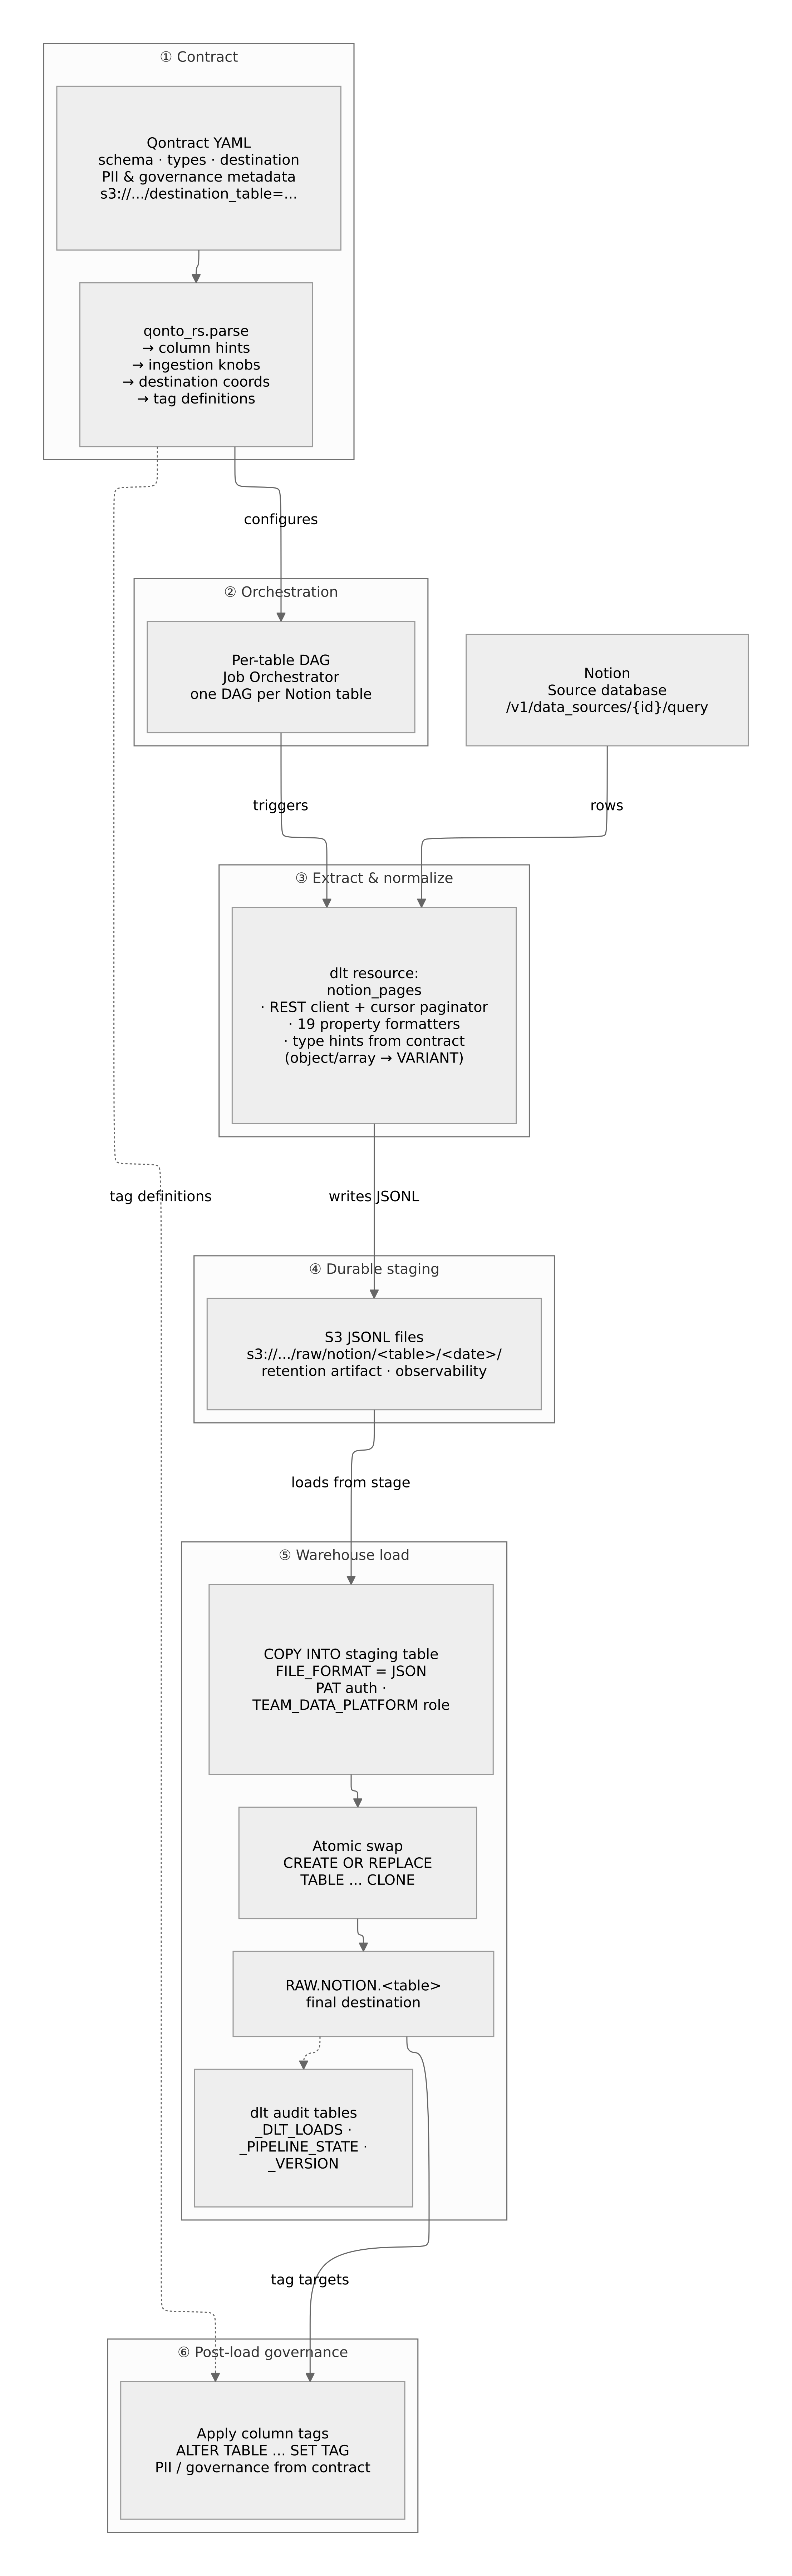
\includegraphics[height=0.95\textheight]{imgs/notion_archi.png}
\caption{End-to-end architecture of the Notion$\rightarrow$dlt pipeline.}
\label{fig:notion-archi}
\end{figure}

The pivotal function, \texttt{build\_resource\_from\_contract()}, is \emph{pure} (no I/O): it reads the YAML contract and derives from it the list of fields, the dlt \emph{column hints} via a \texttt{yaml\_to\_dlt\_columns()} translator, the table name and the primary key (the contract's, otherwise falling back to \texttt{id}), then builds the dlt resource, applying those hints with the ``replace'' write disposition. Listing~\ref{lst:notion-parse} shows this parsing: it is exactly the code behind the type mapping introduced in Chapter~\ref{ch:context} (Table~\ref{tab:type-map}).

\begin{lstlisting}[language=Python,caption={How a Qontract is parsed into a typed dlt resource.},label={lst:notion-parse}]
# contracts.py -- translate ONE contract field into a dlt column hint
def yaml_field_to_dlt_column(prop):
    # ODCS v3.1.0: resolve physicalType first (narrow, e.g. timestamp_ntz),
    # then fall back to logicalType (abstract, e.g. timestamp).
    if prop.physical_type in _LOGICAL_TYPE_TO_DLT:
        column = dict(_LOGICAL_TYPE_TO_DLT[prop.physical_type])
    else:
        column = dict(_LOGICAL_TYPE_TO_DLT[prop.logical_type])
    column["nullable"] = True            # legacy made every column nullable
    if prop.primary_key:
        column["primary_key"] = True
        column["nullable"] = False       # PK stays NOT NULL (Notion page id)
    return column

def yaml_to_dlt_columns(properties):
    # key by normalized (lowercased) name so dlt matches columns at load time
    return {normalize_column_name(p.name): yaml_field_to_dlt_column(p)
            for p in properties}

# main.py -- wire the parsed contract into a configured dlt resource (pure)
def build_resource_from_contract(contract, access_token, ...):
    schema      = contract.schema[0]
    source_id   = contract.get_custom("ingestion.resource_id")
    page_size   = contract.get_custom("ingestion.page_size")   # e.g. 50
    fields      = [p.name for p in schema.properties]
    columns     = yaml_to_dlt_columns(schema.properties)       # type hints
    primary_key = next((normalize_column_name(p.name)
                        for p in schema.properties if p.primary_key), "id")
    resource = notion_pages(source_id, access_token, fields, page_size)
    return resource.apply_hints(
        table_name=schema.name.lower(),
        columns=columns,               # types + nullability from the contract
        primary_key=primary_key,
        write_disposition="replace",   # full refresh -> atomic swap
    )
\end{lstlisting}

Two design choices in this parsing are worth noting. Resolving \texttt{physicalType} \emph{before} \texttt{logicalType} is what lets a \texttt{created\_time} field (\texttt{logicalType: timestamp}, \texttt{physicalType: timestamp\_ntz}) produce a \texttt{TIMESTAMP\_NTZ} column rather than a timezone-aware one; and forcing every column \texttt{nullable} (except the primary key) mirrors the legacy CSV$\rightarrow$VARCHAR pipeline, so a contract's \texttt{required:\ true} never aborts the load on the first NULL.

Everything then starts from \emph{a single call}, \texttt{pipeline.run()}, monolithic from the outside but internally chaining three phases:

\begin{enumerate}
  \item \textbf{Extract}: the resource queries \texttt{/v1/data\_sources/\{id\}/query} via dlt's REST client and its paginator. \emph{Pagination is delegated to the library}, which stops on the documented \texttt{has\_more=false}. \textbf{This is the underlying fix for the silent truncation}: an in-house paginator may terminate incorrectly and truncate silently. Records are buffered then written to local JSONL and nothing touches Snowflake yet.
  \item \textbf{Normalize}: dlt re-reads the JSONL, applies the contract's column hints, and rewrites the files. The format is forced to JSONL so that semi-structured columns land as \emph{native} VARIANT/ARRAY.
  \item \textbf{Load}: the only phase that talks to Snowflake. dlt generates the SQL sequence of Listing~\ref{lst:notion-sql}.
\end{enumerate}

\begin{lstlisting}[language=SQL,caption={SQL sequence generated by dlt during the load phase.},label={lst:notion-sql}]
-- 1) staging table typed by the contract's column hints
CREATE TABLE IF NOT EXISTS RAW.NOTION_STAGING.<TABLE> (...);
-- 2) bulk load from the JSONL on S3 (external stage)
COPY INTO RAW.NOTION_STAGING.<TABLE> FROM @<s3_stage>/... FILE_FORMAT=(TYPE=JSON);
-- 3) atomic swap (staging-optimized + enable_atomic_swap)
ALTER TABLE RAW.NOTION.<TABLE> SWAP WITH RAW.NOTION_STAGING.<TABLE>;
-- 4) load audit row
INSERT INTO RAW.NOTION._DLT_LOADS (load_id, schema_name, status, inserted_at) VALUES (...);
\end{lstlisting}

A methodological point I made sure to understand precisely: \emph{I write none of these queries}. dlt produces them from the destination configuration (atomic swap, ``staging-optimized'' strategy) and the column hints. My work consisted in \emph{choosing the right safe defaults} and \emph{constraining} the framework, not in rewriting the plumbing.

\section{The real challenge: byte-for-byte parity with the legacy}

The dlt pipeline was the easy part. The central technical difficulty was elsewhere: \textbf{producing output \emph{identical} to the legacy system's}, so that no downstream dbt model would break at cutover time. Left to its defaults, dlt would have drifted along several axes; I had to constrain it everywhere (Table~\ref{tab:parity}).

\begin{table}[H]
\centering\small
\renewcommand{\arraystretch}{1.3}
\begin{tabularx}{\textwidth}{@{}p{2.9cm}X@{}}
\toprule
\textbf{Axis} & \textbf{Constraint imposed for parity} \\
\midrule
Column naming & dlt normalises to \emph{snake\_case} (strips the trailing \texttt{\_}, collapses \texttt{\_\_}). I wrote a custom naming convention (\texttt{naming.py}, imposed before importing dlt) that reproduces exactly the legacy cleaning, transliterates accents/emojis and \emph{suffixes Snowflake reserved words with a} \texttt{\_} (\texttt{table}, \texttt{on}, \texttt{start}\dots). \\
Types & Contract $\rightarrow$ dlt-hints translator routing first by the \emph{physical type} (ODCS). \\
Values & Coercion by Notion property type: dates reduced to the local day, timestamps as local wall-clock time (offset stripped), integers rounded, decimals as \texttt{NUMBER(38,6)}, semi-structured kept native. \\
Nullability & All columns forced to \emph{nullable} (except the primary key), because the legacy load made everything nullable. \\
S3 layout & Same date partitioning as the legacy, preserving load history. \\
\bottomrule
\end{tabularx}
\caption{The five parity axes constrained to make the cutover invisible downstream.}
\label{tab:parity}
\end{table}

This is the project's key lesson: the real difficulty was not ``using dlt'', but \emph{guaranteeing zero drift} of schema or value relative to production, so that the cutover would be transparent to the hundreds of downstream dbt models. Each constraint in Table~\ref{tab:parity} corresponds to a real parity bug, diagnosed and then fixed, often at the cost of a fine investigation of both systems' behaviour.

\section{Two mechanisms re-implemented around dlt}

dlt provides pagination, staging and the swap ``for free'', but it does not reproduce two behaviours of the legacy swap that had to be preserved. I coded them around \texttt{pipeline.run()}.

\paragraph{(a) Grant preservation on the swap.} Snowflake's \texttt{SWAP WITH} operation \emph{also exchanges grants}: after the swap, consumer roles (dbt, BI tools) would lose access on every run. I reproduced the legacy operator's behaviour: read the grants (\texttt{SHOW GRANTS}) \emph{before} the load, then \emph{re-apply} them one by one \emph{after} the swap.

\paragraph{(b) Schema reconciliation on contract drift.} The ``replace'' disposition replaces \emph{rows}, not the \emph{schema}: dlt never re-types an existing column. If a contract re-types a field (for example \texttt{text} $\rightarrow$ \texttt{array}), dlt would keep the old type indefinitely. I wrote a drift detector (\texttt{DESC TABLE} compared to the contract's expected types) which, on a re-typing or a removed column, switches the run to a rebuild mode; otherwise the interruption-free atomic swap is preserved. The mechanism is \emph{fail-safe by default} (any introspection error $\rightarrow$ no destructive rebuild) and \emph{self-resolving}.

\section{The zero-downtime production cutover}

The trickiest part was not writing the pipeline, but \emph{cutting over production} without breaking the dbt consumers or the Airflow sensor logic. I achieved it through a \emph{sequence of backward-compatible PRs} in \texttt{qonto-airflow} (Figure~\ref{fig:cutover}).

\begin{figure}[H]
\centering
\begin{tikzpicture}[font=\sffamily\scriptsize,node distance=3mm,
  pstep/.style={rectangle,rounded corners=2pt,draw=qaccent!60,fill=qaccent!8,align=center,inner sep=4pt,text width=2.5cm,minimum height=12mm},
  arr/.style={-{Stealth[length=1.6mm]},draw=qgray,thick}]
\node[pstep] (s1) {\textbf{\#1419}\\wire the dlt loader \emph{alongside} the old one};
\node[pstep,right=of s1] (s2) {\textbf{\#1513}\\cutover: dlt takes over \texttt{RAW.NOTION} (+ transitional shims)};
\node[pstep,right=of s2] (s3) {\textbf{\#1511}\\repoint the sensors to the \texttt{load} task};
\node[pstep,right=of s3] (s4) {\textbf{\#1529}\\remove the transitional shims};
\node[pstep,right=of s4] (s5) {\textbf{\#1536}\\decommission the operator and dependency};
\draw[arr] (s1)--(s2); \draw[arr] (s2)--(s3); \draw[arr] (s3)--(s4); \draw[arr] (s4)--(s5);
\end{tikzpicture}
\caption{Zero-downtime cutover sequence, from wiring in parallel to decommissioning.}
\label{fig:cutover}
\end{figure}

The detail that makes the difference: the sensors always targeted \texttt{raw.notion.<table>}, with table name and cadence \emph{unchanged} so downstream saw nothing happen. That is the very definition of a zero-downtime migration. The final step removed the legacy operator (about 300 lines) and its tests (about 550 lines), an orphaned Airflow \emph{pool}, an obsolete environment \emph{mapping}, and above all the \texttt{notion-client} dependency from the base image.

\begin{keybox}[Results and evaluation]
\begin{itemize}
  \item \textbf{Silent truncation eliminated by construction}: pagination delegated to the library and a \texttt{\_dlt\_loads} audit table on every load.
  \item \textbf{Coupling removed}: no more \texttt{notion-client} dependency in the Airflow base image.
  \item \textbf{Cutover with no downtime and no dbt regression}: byte-for-byte parity verified (names, types, nullability, time zones, S3 layout).
  \item \textbf{Reduced debt}: removal of the three-operator chain, the orphaned pool and the associated tests (on the order of 850 lines removed on the \texttt{qonto-airflow} side).
  \item \textbf{Added robustness}: grants preserved on the swap, schema drift auto-reconciled, a dedicated per-module test suite.
\end{itemize}
\end{keybox}

\begin{contribbox}
I carried this project end to end: incident analysis, comparison of approaches, full development of the dlt job and its modules, resolution of the five parity axes, re-implementation of grants and schema reconciliation, and steering of the cutover PR sequence into production (\#1419 to \#1536). I also spotted two latent bugs in the legacy code while reading it (a loop variable used outside its loop, and an error on an empty Notion database). Ownership of the system was then transferred to the Data Engineering team.
\end{contribbox}
